\documentclass[12pt]{report}

\usepackage{commands}


\begin{document}

\large

\begin{center}
 Math 585 Homework 4\\
 Due Soon\\
 By Marvyn Bailly\\
\end{center}

\normalsize

\hrule

%---------------%
%---Problem 1---%
%---------------%

%--status--$

\begin{problem}
    T1: Prove the convergence of the backward Euler method, that is, the global error $E_n = y_n-y(t_n)$ is $\O(h)$ as $h \to 0$ for all $n = 0, \dots, N$, $h = (b - a)/N$. Here $y(t_n)$ is the exact solution to
    $y'(t) = f(t, y)$ at $t_n = a + nh$, and $y_n$ is the numerical solution obtained by the backward Euler method: $y_{n+1} = y_n + f(t_{n+1}, y_{n+1})$, with $y_0 = y(a)$ taking the exact initial condition.
    (Hint: You may follow the convergence proof of the forward Euler method I did in class. The inequality $1 - x \leq e^{-x} , x \geq 0$ might be useful.)
\end{problem}

\begin{solution}

    \noindent
    Consider the Backward Euler method that is defined by
    \[ 
        y_{n+1} = y_n + hf(t_{n+1},y_{n+1}),
    \]
    and we wish to show that the global error $E_n = y_n-y(t_n)$ is $\O(h)$ as $h \to 0$ for all $n = 0, \dots, N$, $h = (b - a)/N$, where $h = (b - a)/N$, $y(t_n)$ is the exact solution, and $y_n$ is the numerical solution obtained by Backward Euler with the initial condition $y_0 = y(a)$. First we define an auxiliary function to be
    \[ 
        \bar{y}_{n+1} = y(t_n) + hf(t_{n+1},y(t_{n+1})),
    \]
    and observe that
    \[ 
        y(t_{n+1}) - \bar{y}_{n+1} = y(t_{n+1}) -y(t_n) + hf(t_{n+1},y(t_{n+1})) = h T_n,
    \] 
    where $T_n$ is the local truncation error of Backward Euler at the $n$th step which is given by
    \[ 
        T_n = \frac{y(t_{n+1}) - y(t_n)}{h} - f(t_{n+1}, y_{n+1}) = \frac{-y''(\xi_n)}{2}h,
    \]
    where $\xi_n \in [t_n, t_{n+1}]$. Assuming that $M = \max_{a \leq t \leq b}|y''|$ gives that maximum truncation error over all steps is
    \[ 
        T = \max_{0 \leq n \leq N}|E_n| = \frac{M}{2}h.
    \]
    Using these facts, observe that
    \begin{align*}
        |E_{n+1}| &= |y_{n+1} - y(t_{n+1})|\\
        &= \abs{ y_{n+1} - \bar{y}_{n+1} + \bar{y}_{n+1} - y(t_{n+1}) }\\
        &\leq \abs{y_{n+1} - \bar{y}_{n+1}} + \abs{\bar{y}_{n+1} - y(t_{n+1})}\\
        &= \abs{y_n + hf(t_{n+1},y_{n+1}) - y(t_n) - hf(t_{n+1},y(t_{n+1}))} + \abs{\bar{y}_{n+1} - y(t_{n+1})}\\
        &= \abs{y_n - y(t_n)} + h\abs{f(t_{n+1},y_{n+1}) - f(t_{n+1},y(t_{n+1}))} + \abs{\bar{y}_{n+1} - y(t_{n+1})}.
    \end{align*}
    Recall that $f$ is known to be Lipschitz and thus $\abs{f(t_{n+1},y_{n+1}) - f(t_{n+1},y(t_{n+1}))} \leq L \abs{y_{n+1} - y(t_{n+1})}.$ Then we have that
    \begin{align*}
        |E_{n+1}| &= \abs{y_n - y(t_n)} + hL\abs{y_{n+1} - y(t_{n+1})} + \abs{\bar{y}_{n+1} - y(t_{n+1})}\\
        &\leq |E_n| + hL |E_{n+1}| + hT\\
        \implies |E_{n+1}| &\leq \paren{\frac{1}{1 - hL}}\paren{|E_n| + hT},
    \end{align*}
    where we restrict $hL < 1$. Repeating this process for $E_{n-1},\dots,E_{0}$ gives
    \begin{align*}
        |E_{n+1}| &\leq \paren{\frac{1}{1 - hL}}\paren{|E_n| + hT}\\
        & \leq \paren{\frac{1}{1 - hL}}\paren{\paren{\frac{1}{1 - hL}}\paren{|E_{n-1}| + hT} + hT}\\
        &= \paren{\frac{1}{1 - hL}}^2|E_{n-1}| + \paren{\frac{1}{1 - hL}}^2hT + \paren{\frac{1}{1 - hL}}hT\\
        &= \paren{\frac{1}{1 - hL}}^2 \paren{|E_{n-1}| + hT(1 + (1 -hL))}\\
        &~~\vdots\\
        &= \paren{\frac{1}{1 - hL}}^{n+1} \paren{|E_{0}| + hT(1 + (1 -hL) + \dots +(1-hL)^n)}.
    \end{align*}
    Noticing that we have a partial geometric sum of the form $\sum_{i = 0}^n (1 - hL)^i = \frac{1-(1-hL)^{n+1}}{hL}$ and re-indexing reduces the inequality to
    \begin{align*}
        |E_{n}| &\leq  \paren{\frac{1}{1 - hL}}^{n} \paren{|E_{0}| + \frac{T}{L}\paren{1 - hL}^n}\\ 
        &= \paren{\frac{1}{1 - hL}}^{n} \paren{\frac{T}{L}\paren{1 - hL}^n}\\
        &= \frac{T}{L}\paren{\paren{\frac{1}{1 - hL}}^{n} - 1}
    \end{align*}
    where $|E_{0}| = 0$ as we know $y_0 = y(a)$ is the exact initial condition. Now we wish to bound $(1 - hL)^{-n}$. Note that since $n = 0, \dots, N$ and $hL < 1$, we have
    \begin{align*}
        |E_{n}| &\leq \frac{T}{L}\paren{\paren{1 - hL}^{-n} - 1}\\ 
        &\leq \frac{T}{L}\paren{\paren{1 - hL}^{-N} - 1}\\ 
        &= \frac{T}{L}\paren{\paren{1 - hL}^{\frac{-(b-a)L}{hL}} - 1}\\ 
        &= \frac{T}{L}\paren{\paren{ \paren{1-hL}^{-\frac{1}{hL}}}^{(b-a)L} - 1}
    \end{align*} 
    All that is left to do is bound $\paren{1-hL}^{-\frac{1}{hL}}$. Let's consider the function $g(x) = (1 - x)^{-1/x}$. We know that $g(x)$ is strictly increasing on $(0,1)$ and blows up at $x = 1$. Since we restricted $x = hL < 1$, we have that $x < \frac{1}{1+\eps} \leq 1$ for some $\eps \geq 0$. Thus $g(x)$ is bounded on $(0,1)$ by $g(\frac{1}{1+\eps}) = (1 - \frac{1}{1 + \eps})^{-\frac{1}{1 + \eps}}$. Using this fact, we get that
    \begin{align*}
        |E_{n}| &\leq \frac{T}{L}\paren{\paren{1 - \frac{1}{1 + \eps}}^{-\frac{(b-a)L}{1 + \eps}} - 1}\\
        &= \frac{Mh}{2L}\paren{\paren{1 - \frac{1}{1 + \eps}}^{-\frac{(b-a)L}{1 + \eps}} - 1} = \O(h).
    \end{align*}
    Therefore the convergence of the backward Euler method is $\O(h)$.
\end{solution}

%----------------------------------------------------------------------------------------------------%
%\vskip 20pt
\newpage

%---------------%
%---Problem 2---%
%---------------%

%--status--$

\begin{problem}
    Derive the two-step Adams-Moulton formula
    \[ 
        y_{n+1} = y_n + \frac{h}{12} \paren{5f(t_{n+1},y_{n+1}) + 8f(t_n, y_n) - f(t_{n-1},y_{n-1})}.   
    \] 
\end{problem}

\begin{solution}
    
    \noindent
    We wish to derive the two-step Adams-Moulton formula. Recall that the Adam's family is given by
    \[ 
        y(t_{n+1}) = y(t_n) + \int_{t_n}^{t_{n+1}}f(t,y(t))dt = y(t_n)+ \int_{t_n}^{t_{n+1}}p(t)dt,
    \]
    where $f(t,y(t))$ is approximated by an interpolating polynomial $p(t)$. Since we wish to derive the two-step Adams-Moulton, which is an implicit multistep method, we use the points $t_{n+1}, t_n, \and t_{n-1}$ corresponding to $f_{n+1}, f_n, \and f_{n-1}$ respectively. Then we have the interpolating polynomial to be
    \begin{align*}
        p_3(t) &= f_{n-1} + \frac{f_n - f_{n-1}}{h}(t - t_n) + \paren{\frac{\frac{f_{n+1} - f_n}{h} - \frac{f_n - f_{n-1}}{h}}{2h}}(t - t_{n-1})(t - t_n)\\
        &= f_{n-1} + \frac{f_n - f_{n-1}}{h}(t - t_n) + \paren{\frac{f_{n+1} - 2f_n + f_{n-1}}{2h^2}}\paren{t^2 - tt_n - tt_{n-1} + t_{n-1}t_n}\\
        &= f_{n-1} + \frac{f_n - f_{n-1}}{h}(t - t_n) + A\paren{t^2 - tt_n - tt_{n-1} + t_{n-1}t_n}.
    \end{align*} 
    Then we have that
    \[ 
        y(t_{n+1}) = y(t_n)+ \int_{t_n}^{t_{n+1}}p_3(t)dt,
    \]
    and all that is left to do is compute the integral. Observe that
    \begin{align*}
        \int_{t_n}^{t_{n+1}}p_3(t)dt &= \int_{t_n}^{t_{n+1}} f_{n-1} + \frac{f_n - f_{n-1}}{h}(t - t_n) + A\paren{t^2 - tt_n - tt_{n-1} + t_{n-1}t_n} \dt{t}\\
        &= \frac{h}{2}\paren{3f_n - f_{n-1}} + \int_{t_n}^{t_{n+1}} At^2 - Att_n - Att_{n-1} + At_{n-1}t_n \dt{t}\\
        &= \frac{h}{2}\paren{3f_n - f_{n-1}} + \left[ \frac{At^3}{3} - \frac{At^2}{2}t_n - \frac{At^2}{2}t_{n-1} + Att_n t_{n-1}\right]_{t_n}^{t_{n+1}} \\
        &= \frac{h}{2}\paren{3f_n - f_{n-1}} + \frac{A}{6}\left[ 2t_{n+1}^3 - 3t_{n-1}t_{n+1}^2 - et_n t_{n+1}^2 + 6t_{n-1}t_n y_{n+1} + t_n^3 - 3t_{n-1}t_n^2\right]\\
        &= \frac{h}{2}\paren{3f_n - f_{n-1}} + \frac{A}{6}\left[ (-3t_{n-1} + t_n + 2t_{n+1})(t_n - t_{n+1})^2\right]\\
        &= \frac{h}{2}\paren{3f_n - f_{n-1}} + \frac{A}{6}\left[ 5h \cdot h^2\right]\\
        &=  \frac{h}{2}\paren{3f_n - f_{n-1}} + \paren{\frac{f_{n+1} - 2f_n + f_{n-1}}{12h^2}}\paren{5h^3}\\
        &= \frac{h}{2}\paren{3f_n - f_{n-1}} + \frac{h}{12}\paren{f_{n+1} - 2f_{n} + f_{n-1}}\\
        &= \frac{h}{12}\paren{5f(t_{n+1},y_{n+1}) + 8f(t_n, y_n) - f(t_{n-1},y_{n-1})}.
    \end{align*}
    Therefore we have found the two-step Adams-Moulton formula to be
    \begin{align*}
        y(t_{n+1}) &= y(t_n)+ \int_{t_n}^{t_{n+1}}p_3(t)dt\\
        &= y(t_n) + \frac{h}{12}\paren{5f(t_{n+1},y_{n+1}) + 8f(t_n, y_n) - f(t_{n-1},y_{n-1})}
    \end{align*}
\end{solution}

%----------------------------------------------------------------------------------------------------%
%\vskip 20pt
\newpage

%---------------%
%---Problem 3---%
%---------------%

%--status--$

\begin{problem}
    Show that the local truncation error of the Adams-Moulton method derived above is $\O(h^3).$
\end{problem}

\begin{solution}

    \noindent
    Recall the two-step Adams-Moulton formula is given by
    \[ 
        y_{n+1} = y_n + \frac{h}{12} \paren{5f(t_{n+1},y_{n+1}) + 8f(t_n, y_n) - f(t_{n-1},y_{n-1})},
    \] 
    and has local truncation error of
    \[ 
        T_n = \frac{1}{h}\paren{y(t_{n+1}) - y(t_n)} - \frac{1}{12}\paren{5y'(t_{n+1}) + 8y'(t_n) - y'(t_{n-1})}.
    \]
    Observe the following Taylor expansions
    \begin{align*}
        y(t_{n+1}) &= y(t_n) + hy'(t_n) + \frac{h^2}{2}y''(t_n) + \frac{h^3}{6}y''' + \O(h^4),\\
        y(t_{n-1}) &= y(t_n) - hy'(t_n) + \frac{h^2}{2}y''(t_n) - \frac{h^3}{6}y''' + \O(h^4),\\
        y'(t_{n+1})' &= y'(t_n) + hy''(t_n) + \frac{h^2}{2}y'''(t_n) + \O(h^3),\\
        y'(t_{n-1})' &= y'(t_n) - hy''(t_n) + \frac{h^2}{2}y'''(t_n) + \O(h^3).
    \end{align*}
    Then plugging the expansions into the local truncation error yields
    \begin{align*}
        T_n &= \frac{1}{h} \paren{ \paren{y(t_n) + hy'(t_n) + \frac{h^2}{2}y''(t_n) + \frac{h^3}{6}y''' + \O(h^4)} - y(t_n)}\\
        &- \frac{1}{12} \left( 5\paren{y'(t_n) + hy''(t_n) + \frac{h^2}{2}y'''(t_n) + \O(h^3)} + 8y'(t_n) \right.\\ 
        &\left. -\paren{y'(t_n) - hy''(t_n) + \frac{h^2}{2}y'''(t_n) + \O(h^3)} \right)\\
        &= \paren{y'(t_n) + \frac{1}{2}h y''(t_n) + \frac{1}{6}h^2y'' + \O(h^3)} - \frac{1}{12}\paren{12y'(t_n) + 6hy''(t_n) + 2h^2y''' + \O(h^3)}\\
        &= \O(h^3).
    \end{align*}
    Thus we have shown that the local truncation error of the two-step Adams-Moulton formula is $\O(h^3)$. 


\end{solution}

%----------------------------------------------------------------------------------------------------%
%\vskip 20pt
\newpage

%---------------%
%---Problem 4---%
%---------------%

%--status--$

\begin{problem}
    Show that the implicit midpoint method given below is A-stable.
    \[ 
        y_{n+1} = y_n + hf(t_{n + 1/2},y_{n + 1/2}), ~~~ t_{n + 1/2} = t_n + h/2, ~~~ y_{n + 1/2} = \frac{y_n + y_{n+1}}{2}.
    \]
\end{problem}

\begin{solution}

    \noindent
    We wish to show that the implicit midpoint method
    \[ 
        y_{n+1} = y_n + hf(t_{n + 1/2},y_{n + 1/2}), ~~~ t_{n + 1/2} = t_n + h/2, ~~~ y_{n + 1/2} = \frac{y_n + y_{n+1}}{2},
    \]
    is A-stable. To do so, let's apply the method to the test problem
    \[ 
        y' = \lambda y,
    \]
    which gives
    \[ 
        y_{n+1} = y_n + h\lambda y_{n+1/2} = y_n + h\lambda\paren{\frac{y_n + y_{n+1}}{2}}.
    \]
    Now solving for $y_{n+1}$ gives
    \begin{align*}
        y_{n+1} &= y_n + \frac{h}{2}\lambda y_n + \frac{h}{2}\lambda y_{n+1}\\
        y_{n+1} -\frac{h}{2}\lambda y_{n+1} &= y_n + \frac{h}{2}\lambda y_n\\
        \implies y_{n+1} &= \frac{y_n + \frac{h}{2}\lambda y_n}{1 - \frac{1}{2}h\lambda}.\\
    \end{align*}
    Now if we let $z = \lambda h = a + ib$ and look at the absolute stability of the method yields
    \begin{align*}
        \abs{ \frac{2 + z}{2 - z}} &\leq 1\\
        \abs{ \frac{2 + a + ib}{2 - a - ib}} &\leq 1\\
        \abs{2 + a + ib}^2 &\leq \abs{2 - a - ib}^2\\ 
        \paren{2 + a}^2 + b^2 &\leq \paren{2 - a}^2 + b^2\\ 
        \paren{2 + a}^2&\leq \paren{2 - a}^2\\
        4 + 4a + a^2 &\leq 4 - 4a + a^2\\
        8a &\leq 0\\
        a &\leq  0,\\
        \implies \text{Re}(z) &\leq 0.
    \end{align*}  
    Thus we have that the region of absolute stability is $\text{Re}(z) \leq 0$ which means that the implicit midpoint method is A-stable.



\end{solution}

%----------------------------------------------------------------------------------------------------%
%\vskip 20pt
\newpage

%---------------%
%---Problem 5---%
%---------------%

%--status--$

\begin{problem}
    C1: Solve the initial value problem
    \[ 
        y'(t) = - \frac{1}{t^2} - \frac{y}{t} - y^2, ~~~ 1 \leq t \leq 2, ~~~ y(1) = -1,
    \]
    \begin{enumerate}
        \item [(a)] using the forward Euler method;
        \item [(b)] using the improved Euler method;
        \item [(c)] using the classical fourth-order Runge-Kutta method.
    \end{enumerate}
    Choose appropriate time steps $h$ and demonstrate the convergence order for each method. You may use MATLAB \verb+ode45+ to generate an “accurate” solution for reference.
\end{problem}

\begin{solution}

    \noindent
    Consider the initial value problem
    \[ 
        y'(t) = - \frac{1}{t^2} - \frac{y}{t} - y^2, ~~~ 1 \leq t \leq 2, ~~~ y(1) = -1.
    \]
    The MATLAB script in Listings 1 was used to run the entire problem.

   


    \begin{enumerate}
        \item [(a)]
        

        \begin{figure}[H]
            \begin{subfigure}[b]{0.5\linewidth}
                \centering
                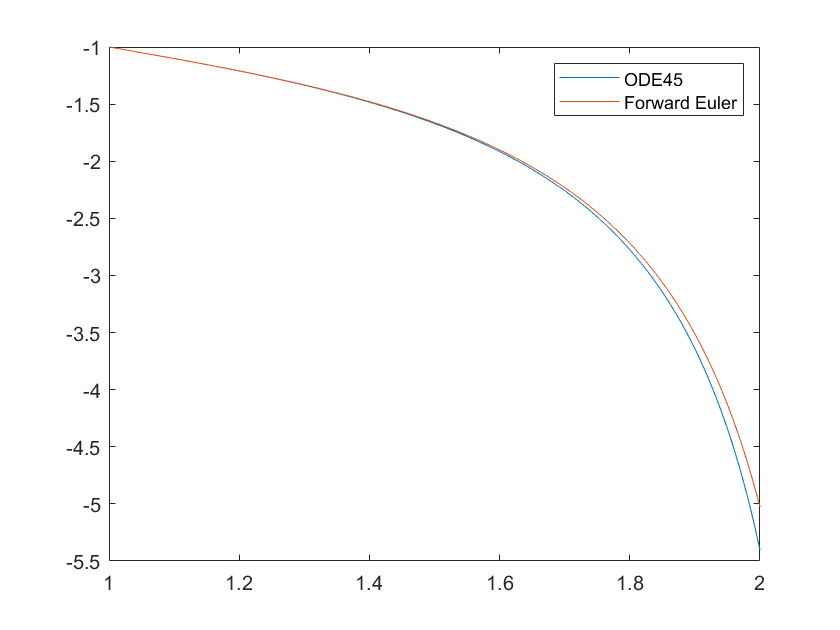
\includegraphics[width=\linewidth]{images/fe1.png}
                \caption{Forward Euler compared to exact solution.}
                \label{fig1:a}
                \vspace{4ex}
            \end{subfigure}%%
            \begin{subfigure}[b]{0.5\linewidth}
                \centering
                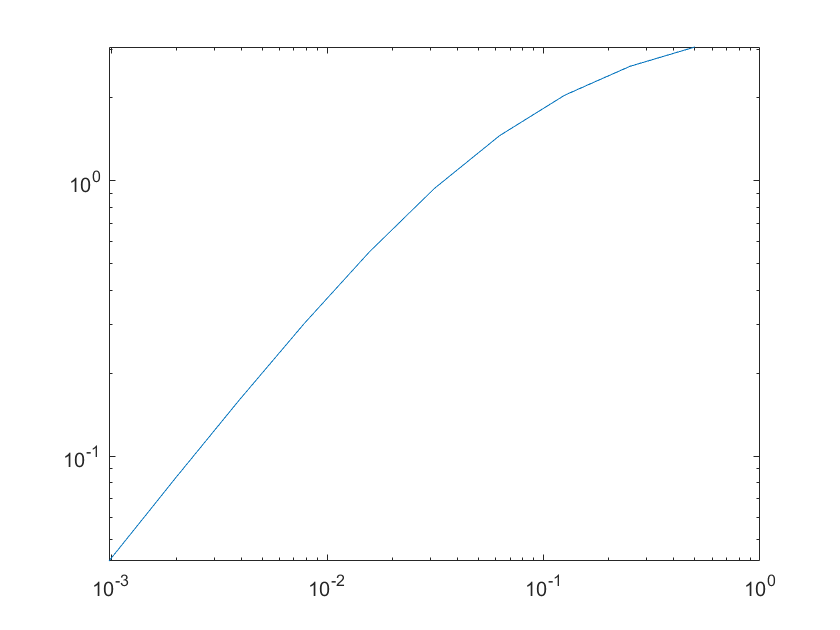
\includegraphics[width=\linewidth]{images/fe2.png}
                \caption{Max error of Forward Euler Method.}
                \label{fig1:b}
                \vspace{4ex}
            \end{subfigure}
            \caption{Plots used to analyze the convergence of the Forward Euler Method.}
            \label{fig1}
        \end{figure}
        First we wish to find the solution using the forward Euler method. I created the code in Listings 2 to preform the forward Euler method and picked $h = 0.01$ to be an appropriate $h$ value. Using MATLAB's \verb+ode45+ function to find the exact solution of the initial value problem, we can plot the approximate solution from forward Euler compared to the exact solution. In figure \ref{fig1:a}, we see that the Forward Euler does not give the best approximation. To study the convergence, we tested $h$ values from $2^-1,\dots,2^{-10}$ and computed the error by using the infinity norm on the difference between the approximate solution and the exact solution. Plotting the max error of each $h$ value on a loglog plot, as seen in figure \ref{fig1:b}, we see that the error linearly reduces with $h$. Using MATLAB's \verb+polyfit+ function, we can find that slope of the line is around $1$ which matches the expected convergence of Forward Euler method $\O(h)$.   


        
        \item [(b)]
        Next we wish to find the solution using the improved Euler method. I created the code in Listings 3 to preform the improved Euler method and picked $h = 0.01$ to be an appropriate $h$ value. Using MATLAB's \verb+ode45+ function to find the exact solution of the initial value problem, we can plot the approximate solution from Improved Euler compared to the exact solution. In figure \ref{fig2:a}, we see that the Improved Euler solution matches the exact solution closely. To study the convergence, we tested $h$ values from $2^-1,\dots,2^{-10}$ and computed the error by using the infinity norm on the difference between the approximate solution and the exact solution. Plotting the max error of each $h$ value on a loglog plot, as seen in figure \ref{fig2:b}, we see that the error linearly reduces with $h$. Using MATLAB's \verb+polyfit+ function, we can find that slope of the line is around $2$ which matches the expected convergence of Improved Euler method $\O(h^2)$.   

        \begin{figure}[H]
            \begin{subfigure}[b]{0.5\linewidth}
                \centering
                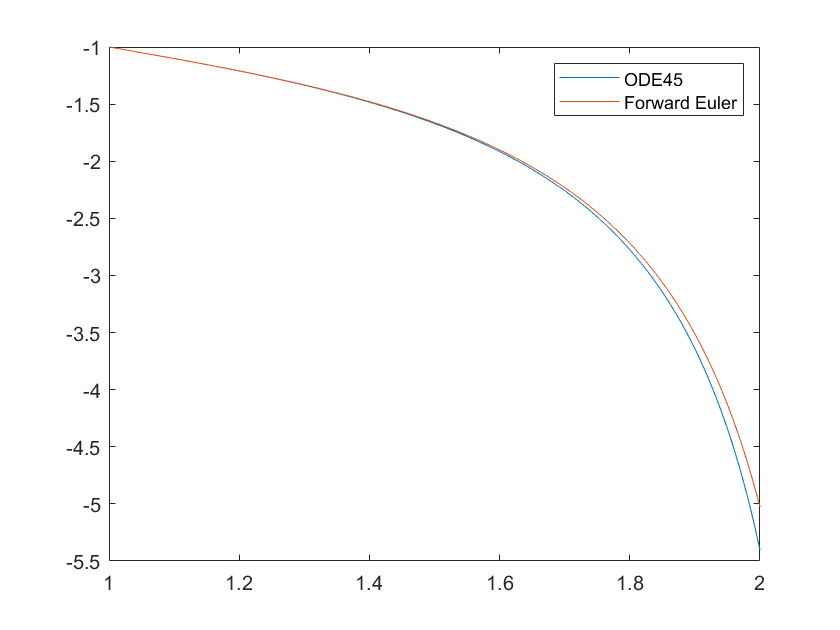
\includegraphics[width=\linewidth]{images/fe1.png}
                \caption{Improved Euler compared to exact solution.}
                \label{fig2:a}
                \vspace{4ex}
            \end{subfigure}%%
            \begin{subfigure}[b]{0.5\linewidth}
                \centering
                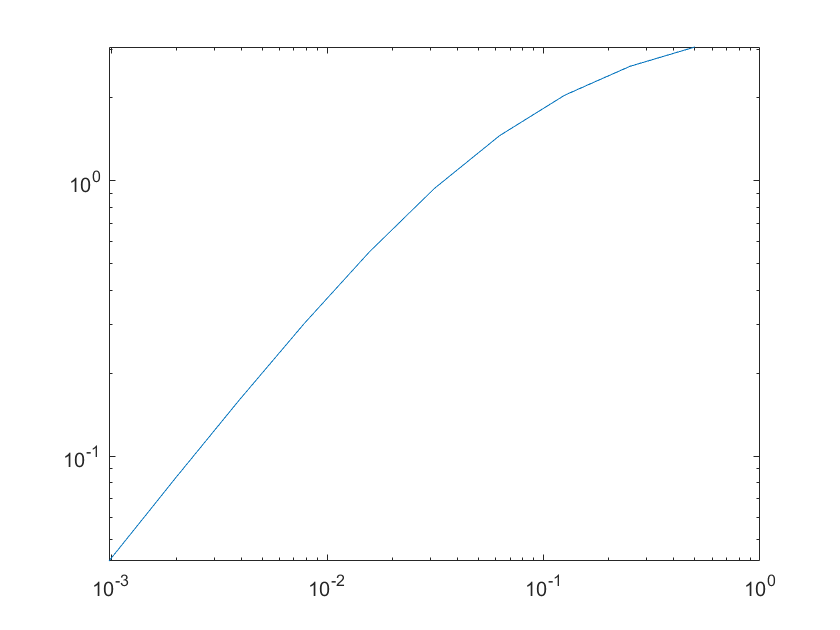
\includegraphics[width=\linewidth]{images/fe2.png}
                \caption{Max error of Improved Euler Method.}
                \label{fig2:b}
                \vspace{4ex}
            \end{subfigure}
            \caption{Plots used to analyze the convergence of the Improved Euler Method.}
            \label{fig2}
        \end{figure}

        


        \item [(c)]
        Next we wish to find the solution using the classical fourth-order Runge-Kutta method. I created the code in Listings 4 to preform the improved Euler method and picked $h = 0.01$ to be an appropriate $h$ value. Using MATLAB's \verb+ode45+ function to find the exact solution of the initial value problem, we can plot the approximate solution from the fourth-order Runge-Kutta compared to the exact solution. In figure \ref{fig3:a}, we see that the fourth-order Runge-Kutta matches the exact solution closely. To study the convergence, we tested $h$ values from $2^-1,\dots,2^{-7}$ and computed the error by using the infinity norm on the difference between the approximate solution and the exact solution. Plotting the max error of each $h$ value on a loglog plot, as seen in figure \ref{fig3:b}, we see that the error linearly reduces with $h$. Using MATLAB's \verb+polyfit+ function, we can find that slope of the line is around $4$ which matches the expected convergence of Forward Euler method $\O(h^4)$.   

        \begin{figure}[H]
            \begin{subfigure}[b]{0.5\linewidth}
                \centering
                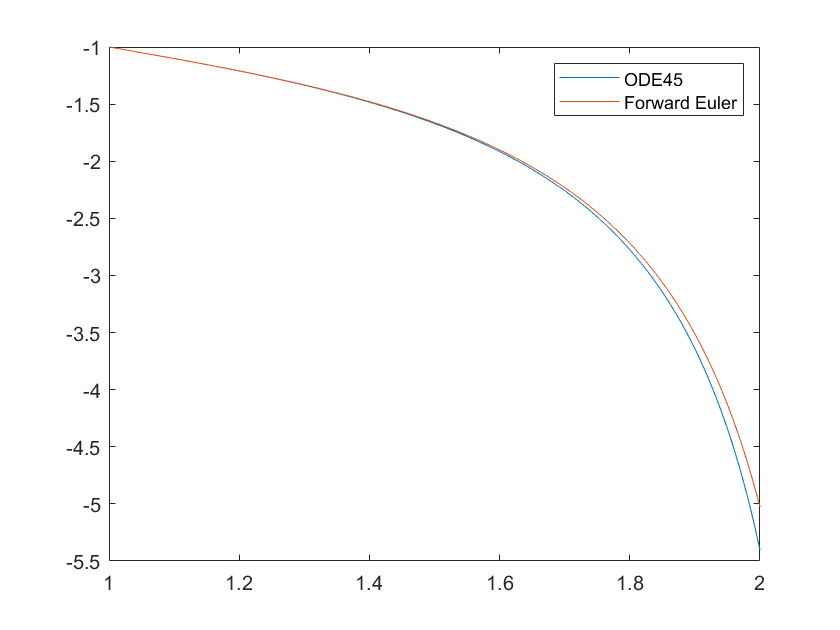
\includegraphics[width=\linewidth]{images/fe1.png}
                \caption{Runge-Kutta compared to exact solution.}
                \label{fig3:a}
                \vspace{4ex}
            \end{subfigure}%%
            \begin{subfigure}[b]{0.5\linewidth}
                \centering
                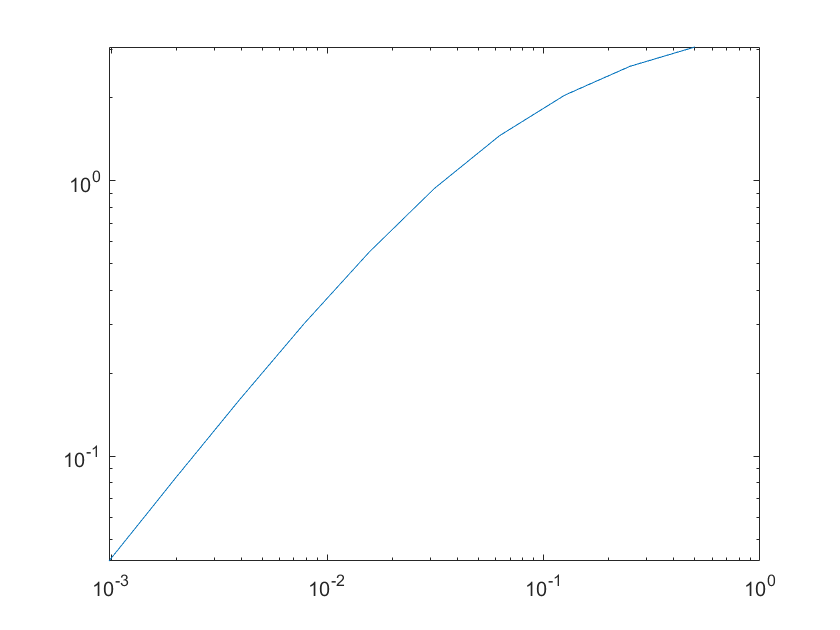
\includegraphics[width=\linewidth]{images/fe2.png}
                \caption{Max error of Runge-Kutta Method.}
                \label{fig3:b}
                \vspace{4ex}
            \end{subfigure}
            \caption{Plots used to analyze the convergence of the Runge-Kutta Method.}
            \label{fig3}
        \end{figure}

        


    \end{enumerate}

    \lstinputlisting[language=MATLAB, caption={\bf Main Script for C1}]{CP1.m}
    \lstinputlisting[language=MATLAB, caption={\bf Forward Euler Method}]{forwardEuler.m}
    \lstinputlisting[language=MATLAB, caption={\bf Improved Euler Method}]{improvedEuler.m}
    \lstinputlisting[language=MATLAB, caption={\bf Classical Fourth-Order Runge-Kutta Method}]{runge.m}
\end{solution}

%----------------------------------------------------------------------------------------------------%
%\vskip 20pt
\newpage

\end{document}